\capitulo{4}{Técnicas y herramientas}

En este capítulo se van a comentar las técnicas y herramientas utilizadas a lo largo del desarrollo del proyecto \textit{software}.

\section{Técnicas}\label{sec:tecnicas}

\subsection{Metodología SCRUM}\label{SCRUM}
\textit{Scrum} es un marco de trabajo que permite el trabajo colaborativo en equipos. Permite que los equipos que trabajan en proyectos con esta metodología se organicen por sí mismos, siendo ellos los que deciden cómo afrontar los problemas que van surgiendo. 

Según \cite{cervone2011understanding}, el modelo \textit{Scrum} se basa en tres componentes principales: roles, procesos y artefactos. El \textit{Scrum Master} es el puesto asumido por el director o gerente del proyecto, o en algunos casos el líder del equipo. Esta figura representa los valores y principios por los que se rige la metodología de \textit{scrum}, manteniendo los valores y buenas prácticas, así como resolviendo los impedimentos que vayan surgiendo a lo largo del desarrollo del proyecto. Habitualmente los equipos están compuestos por entre cinco y diez personas que trabajan en el proyecto a tiempo completo. Siendo este equipo independiente y flexible en cuanto a jerarquía interna, no siendo representado el papel del <<jefe>> dentro de este por la misma persona siempre. Esto genera que el papel cambie en función de las necesidades del propio proyecto, la configuración del equipo cambia únicamente entre iteraciones, o \textit{sprints}, no dentro de los mismos.

\begin{figure}[]
	\centering
	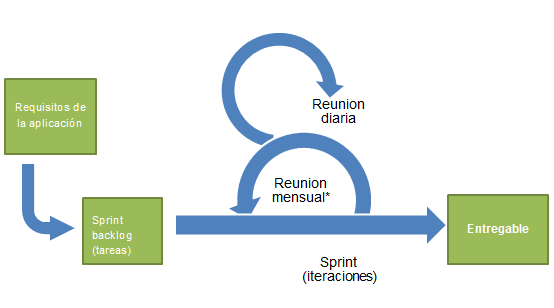
\includegraphics[scale=0.5]{../img/anexos/scrum-overview-es}
	\caption{Metodología \textit{scrum}~\cite{SCRUMWIKI}.}\label{img:scrum-overview}
\end{figure}

\subsubsection{\textit{Sprints}}
Los \textit{sprints} son periodos breves de \textbf{tiempo fijo} en el que el equipo trabaja para completar una cantidad de trabajo preestablecida. Si bien muchas guías asocian los \textit{sprints} a la metodología ágil, asociando la metodología ágil y la metodología seguida en \textit{scrum} como si fueran lo mismo, cuando no lo son. La metodología ágil constituye una serie de principios, y la metodología \textit{scrum} es un marco de trabajo con la única finalidad de conseguir resultados.

A pesar de las similitudes los \textit{sprints} poseen un objetivo subyacente, entregar con frecuencia \textit{software} de trabajo.

\subsubsection{\textit{Sprint meetings}}
Dentro de la metodología \textit{scrum} existen diferentes reuniones que favorecen la agilidad del proyecto y que todo el mundo sepa lo que tiene que hacer en cada momento.
\begin{itemize}
\item \textbf{\textit{Sprint planning meeting.}} Esta reunión puede tener una duración de hasta de un día completo de trabajo. En ella deben de estar presentes todas las partes del proyecto, \textit{i.e.} el \textit{Scrum Master}, el equipo de desarrollo, y el \textit{product owner}. Poseen dos partes, en la primera de ellas se define el \textit{product backlog}, requerimientos del proyecto y se definen los objetivos para el \textit{sprint} que comienza, \textit{i.e.} lo que se espera <<construir>> o completar en el \textit{sprint}. En la segunda parte de la reunión se trabaja en el \textit{sprint backlog}, las tareas que se van a seguir en el \textit{sprint} para completar el objetivo de éste.
\item \textbf{\textit{Daily meeting.}} Debido a que los requerimientos del proyecto no se pueden variar durante la vida de un \textit{sprint}, existen las reuniones diarias que son organizadas por el \textit{Scrum Master} en las que se comenta el trabajo del día previo, lo que se espera de ese día y qué está retrasando o impidiendo a un individuo el proseguir con sus tareas, esta reunión no debe tener una duración de más de quince minutos y se debe realizar <<de pie>>. No es una reunión para ver quién retrasa el proyecto sino para ayudar a quién lo necesite entre todos los miembros del equipo y permitir esa agilidad.
\item \textbf{\textit{Sprint review meeting.}} Reunión fijada al final de cada \textit{sprint} en la cual se hace una puesta en conocimiento de lo que se ha realizado en ese \textit{sprint}, siempre que se pueda se hará una demostración funcional en lugar de una presentación al \textit{product owner}. Esta reunión tiene un carácter informal.
\end{itemize}
 
\subsubsection{Artifacts}
Uno de los componentes más importantes de cara a la metodología \textit{scrum} son los artefactos, o \textit{artifacts} por su nombre en inglés. Estos incluyen el \textit{product backlog}, el \textit{sprint backlog} y los \textit{burn down charts}.
\begin{itemize}
\item \textbf{\textit{Product backlog.}} Lista de trabajo ordenada por las prioridades para el equipo de desarrollo. Es generada a partir de las reuniones de planificación de los \textit{sprints}, contiene los requisitos. Se encuentra actualizado y clasificado en función de la periodicidad asignada a las tareas, pudiendo ser de corto o largo plazo. Aquellas tareas que se deban resolver a corto plazo deberán estar perfectamente descritas antes de asignarlas esta periodicidad, implicando que se han diseñado las historias de usuario completas, así como el equipo de desarrollo ha establecido las estimaciones correspondientes. Los elementos a largo plazo pueden ser abstractos u opacos, conviene que estén estimados en la medida de lo posible para poder tener en cuenta el tiempo que llevará desarrollarla.

Los propietarios del producto dictan la prioridad de los elementos de trabajo en el \textit{product backlog}, mientras que el equipo de desarrollo dicta la velocidad a la que se trabaja el \textit{backlog}~\cite{danradigan2021}.

La estimación es una parte muy importante ya que es lo que permitirá al equipo de desarrollo mantener el ánimo y el trabajo al ritmo deseado. La estimación es realizada en la \textit{sprint planning meeting}, en la que se estima para cada tarea/producto del \textit{product backlog}. No se busca tener un resultado exacto del tiempo que va a llevar al equipo completar esa tarea, sino es una previsión. Para realizar correctamente la estimación se debe tener en cuenta el tamaño y la categoría de la tarea, los puntos de historia que se le van a asignar, así como el número de horas y días que van a ser necesarias para completar la tarea. 

\item \textbf{\textit{Sprint backlog.}} Lista de tareas extraídas del \textit{product backlog} que se han acordado desarrollarse a lo largo de un \textit{sprint}. Este \textit{backlog} es seleccionado por el propio equipo de desarrollo, para ello seleccionan una tarea del \textit{product backlog} y se divide en tareas de menor tamaño y abordables. Aquellas tareas de menor tamaño que el equipo no haya sido capaz de desarrollar previo a la finalización del \textit{sprint} quedarán almacenadas para próximos \textit{sprints} en el \textit{sprint backlog}.
\end{itemize}

\subsubsection{Actores, roles y responsabilidades}
Dentro de un equipo que sigue la metodología \textit{scrum} encontramos diferentes actores, como ya se ha comentado el equipo de desarrollo suele estar compuesto por entre cinco y diez personas, además del \textit{Scrum Master} y el \textit{Product Owner}~\cite{julioroche_2020}.
\begin{itemize}
\item \textbf{\textit{Product Owner.}} Encargado de optimizar y maximizar el valor del producto, es la persona encargada de gestionar las prioridades del \textit{product backlog}. Una de sus principales tareas es la de ser intermediario con los \textit{stakeholders}, partes interesadas, del proyecto; junto con recoger los requerimientos de los clientes. Es habitual que esta figura sea representante del negocio, con lo que aumenta su valor.

Para cada \textit{sprint} debe de marcar el objetivo de éste de manera clara y acordada con el equipo de desarrollo, lo cual hará que el producto vaya incrementando constantemente su valor. Para que todo fluya como debe, esta figura debe tener el <<poder>> de tomar decisiones que afecten al producto.

\item \textbf{\textit{Scrum Master.}} Figura con dos responsabilidades, gestionar el proceso \textit{scrum} y ayudar a eliminar impedimentos que puedan afectar a la entrega del producto.
\begin{enumerate}
\item Gestionar el proceso \textit{scrum}. Su función es asegurarse de que el proceso se lleva a cabo correctamente, facilitando la ejecución de éste y sus mecánicas. Consiguiendo que la metodología sea una fuente de generación de valor.
\item Eliminar impedimentos. Eliminar los problemas que vayan surgiendo a lo largo de los \textit{sprints} con el fin de mantener el ritmo de trabajo dentro de los equipos de desarrollo para poder entregar valor, manteniendo la integridad de la metodología.
\end{enumerate}
\item \textbf{Equipo de desarrollo.} Formado por entre cinco y diez personas encargadas del desarrollo del producto, organizados de forma autónoma para conseguir entregar las tareas del \textit{product backlog} asignadas al \textit{sprint} correspondiente. Para que funcione correctamente la metodología todos los integrantes deben de conocer su rol dentro del equipo, internamente se pueden gestionar como el equipo considere, pero de cara <<hacia fuera>> son un equipo con una responsabilidad.
\end{itemize}

\subsection{Python}
Según~\cite{queespython}, Python es un lenguaje de programación multiplataforma y multiparadigma\footnote{Debido a que soporta parcialmente la orientación a objetos, la programación imperativa, y la programación funcional.}, entre sus principales características se encuentran la legibilidad y limpieza del código. Python es \textit{open source software} por lo que su uso es gratuito~\cite{pythonLICENSE}.

Python fue desarrollado al principio de la década de 1990 por Guido van Rossum en el Stichting Mathematish Centrum, CWI, en el Reino de los Países Bajos. Implementado como el sucesor del lenguaje ABC. Actualmente el lenguaje sigue siendo desarrollado por Guido, junto con contribuciones de muchos otros. El lenguaje está fuertemente influenciado por otros como: ABC, Ada, ALGOL 68, APL, C, C++, CLU, Dylan, Haskell, Icon, Java, Lips, Modula-3, Perl, Standard ML.

El principal objetivo de Python es la automatización de procesos con el fin de minimizar tanto complicaciones como tiempo de desarrollo. Debido a estas dos características, hoy en día Python es el lenguaje de programación más utilizado para desarrollo de todo tipo de aplicaciones, tanto es así que, según las últimas estadísticas recuperadas por PYPL, ver~\cite{pyplindex}, además es el lenguaje de programación sobre el que más tutoriales se buscan en el top buscadores (Google, Bing, DuckDuckGo,\dots). Se aplica en campos tales como:
\begin{itemize}
\item Ciencia de datos. Uso de las bibliotecas de Python desarrolladas para el análisis y visualización de datos.
\item Aprendizaje automático. Dado que Python es un lenguaje de programación tan estable, flexible y sencillo, es perfecto para varios proyectos de aprendizaje automático (ML) e inteligencia artificial (AI). De hecho, Python es uno de los lenguajes favoritos entre los científicos de datos, y hay muchas bibliotecas y paquetes de aprendizaje automático e IA disponibles en Python. 
\item Desarrollo web. Utilizado principalmente en el \textit{back-end} de las aplicaciones web, tanto en la codificación de las funcionalidades, de manera similar a lo que JavaScript permitiría hacer; como encargándose de la conexión con las diferentes bases de datos que puedan estar en producción.
\item Visión artificial y procesamiento de imágenes. 
\item Desarrollo de videojuegos.
\item Medicina y bioinformática.
\item Astronomía.
\end{itemize}

\subsubsection{PEP8}
La abreviación PEP hace referencia a \textit{Python Enterprise Proposal}~\cite{pep8javatpoint}. La escritura de código con la lógica adecuada en un factor clave independientemente del lenguaje de programación en el que se esté trabajando, pero hay muchos más factores que influyen en la calidad del código. El estilo de codificación del programador hace que el código sea mucho más fiable, se debe de tener en cuenta que Python sigue estrictamente la forma de orden y formato de la cadena, \textit{i.e.} tal y como se escribe el código se procesa para su compilación.

PEP8 es un documento el cual proporciona varias directrices para escribir la parte legible en Python. Fue escrito oficialmente en 2001 por Guido van Rossum, Barry Warsaw y Nick Coghlan, con el objetivo principal de mejorar la legibilidad y consistencia del código. Disponible para consulta~\cite{rossum_warsaw_coghlan}.

PEP8 mejora la legibilidad del código, pero ¿a qué se debe que la legibilidad sea tan importante en Python? <<\textit{Code is much more often than it is written.}>>~\cite{guidophrase}. Un fragmento de código puede ser escrito en cuestión de minutos o unas pocas horas, pero una vez escrito no se reescribirá nunca, pero seguramente sí que será leído un número indefinido de veces. Es en ese preciso momento cuando se debe tener una idea del porqué de esa línea de código. El código debe reflejar el significado de cada línea, de ahí el motivo de que la legibilidad sea tan importante.

\subsection{Investigación}
\subsubsection{\textit{Ranking} medio}
En el campo de la estadística, los \textit{rankings} permiten la transformación de datos en función de su posición cuando el conjunto de datos es ordenado.

Para cada conjunto de datos se ordenan los resultados de cada clasificador de tal modo que al mejor clasificador se le da 1, al segundo mejor 2 y así sucesivamente. El \textit{ranking} medio, por lo tanto, es calculado mediante el promedio de los \textit{rankings} de cada clasificador para los distintos conjuntos de datos

\subsubsection{\textit{Test} estadístico}
Mecanismo para tomar decisiones cuantitativas sobre un proceso o una serie de estos. El objetivo es determinar si hay suficientes pruebas para <<rechazar>> una hipótesis sobre el proceso. La conjetura se denomina hipótesis nula. Una hipótesis puede no ser rechazada en tanto en cuanto se desee seguir investigando bajo la suposición de que la hipótesis nula es cierta. O puede ser un resultado decepcionante, que posiblemente indique que aún no se poseen suficientes datos para <<demostrar>> algo rechazando la hipótesis nula~\cite{lucon2018new}~\cite{nist}.

\section{Herramientas}\label{sec:herramientas}
\subsection{UBUMLaaS}\label{UBUMLaaS}
UBUMLaaS surge como una plataforma de \textit{Machine Learning as a Service} basada en los métodos desarrollados tanto por el grupo de investigación ADMIRABLE\footnote{\textit{Advanced Data MIning Research And (Business intelligence | Bioinformatics | Big data) LEarning}.  El objetivo principal del grupo de investigación es el desarrollo de nuevos algoritmos de \textit{ensemble} y la aplicación de técnicas de minería de datos y \textit{pattern matching} a diversos campos como la bioinformática, la clasificación de series temporales y el análisis de datos de alta dimensión~\cite{admirable_intro}.}.

Junto con ellos, se incluyen los desarrollados por el grupo de investigación BEST-AI\footnote{El Grupo de Investigación BEST-AI (Biología, Educación y Salud con Tecnologías Avanzadas Informáticas) de la Universidad de Burgos, centra su actividad investigadora en el desarrollo de nuevos algoritmos de minería de datos e inteligencia artificial y en su aplicación a problemas biológicos, bioinformáticos, sanitarios, medioambientales o educativos.}.

El proyecto permite a terceros, registrados en la plataforma, hacer uso de técnicas de aprendizaje automático en la nube. En una primera instancia fue desarrollado por miembros del grupo ADMIRABLE.

La plataforma, previa a este Trabajo de Fin de Grado, proporciona únicamente soporte a algoritmos de aprendizaje supervisado, estos algoritmos provienen de diversas bibliotecas como son Weka, Meka, Scikit-Learn o los propios algoritmos desarrollados por el grupo ADMIRABLE. Habiendo sido paralizado su soporte a mediados de 2019.

Página web de la herramienta: \url{http://ubumlaas.eu.ngrok.io}

\subsection{Weka}\label{subsec:Weka}
Desarrollado por la Universidad de Waikato~\cite{witten2005practical} es un \textit{open source software} el cual provee de herramientas para el pre-procesado de datos, implementación de algoritmos de \textit{Machine Learning}, y herramientas de visualización, de tal manera que permite desarrollar técnicas de aprendizaje automático y aplicarlas a problemas de minería de datos. 

\begin{figure}
\centering
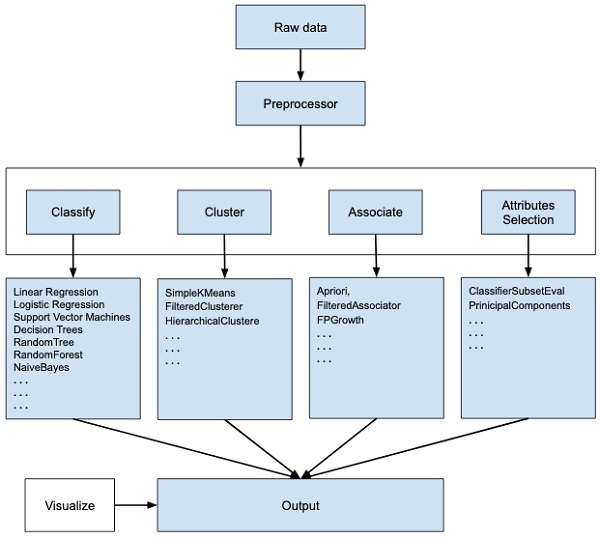
\includegraphics[width=0.75\textwidth]{../img/memoria/weka-summary}
\caption[Resumen de las funcionalidades de Weka.]{Resumen de las funcionalidades de Weka. Imagen recuperada de \url{https://www.tutorialspoint.com/weka/what_is_weka.htm}}\label{fig:whatisweka}
\end{figure}

En la figura~\ref{fig:whatisweka} se observa un diagrama con todas las funcionalidades que ofrece Weka. Para poder utilizar un conjunto de datos en \textit{Machine Learning}, ver sección~\ref{sec:machine-learning}, hay que hacerlos aptos, esto se consigue con el primer paso, el pre-procesado, para ello Weka proporciona una serie de herramientas que permiten limpiar los valores nulos, campos irrelevantes, etcétera. Seguidamente se guardan los datos que han sido pre-procesados en almacenamiento local para aplicar algoritmos de \textit{Machine Learning}\footnote{Esta es una de las principales desventajas de Weka, almacena el conjunto de datos en su totalidad en memoria del sistema, limitando el número de instancias que puede tener un conjunto de datos.}.

En función de qué tipo de modelo de ML se desee aplicar, se selecciona una opción de entre: clasificación, agrupamiento, asociación, o selección de atributos. Weka proporciona una serie de algoritmos para cada modelo, permitiendo su completa parametrización individualizada, de forma que se pueden realizar los experimentos al gusto del investigador. 

Finalmente, Weka proporciona un resultado estadístico del procesamiento del modelo, junto con ello proporciona una herramienta de visualización para inspeccionar los datos. Los distintos modelos pueden aplicarse al mismo conjunto de datos, permitiendo la comparación de los resultados.

Página web de la herramienta: \url{https://waikato.github.io/weka-wiki/}

\subsection{Orange3}
\texttt{Orange} es un \textit{software} de minería de datos basado en componentes. Ofrece un entorno para la creación, de manera rápida y sencilla, prototipos de los algoritmos más comunes de ML y casos de prueba. Un gran número de los componentes que lo conforma están escritos en Python.

Entre los objetivos de \texttt{Orange} figura que sea una plataforma para la experimentación basada en selección, modelado predictivo y sistemas de aprobación. Permitiendo ser utilizada en campos como la bioinformática, el análisis del genoma, biomedicina y la enseñanza. Desde el punto de vista de la educación ofrece un apoyo en la enseñanza de la minería de datos y el aprendizaje automático.

Página web de la herramienta: \url~{https://orangedatamining.com/}


\subsection{PyCharm}

PyCharm es uno de los IDEs\footnote{Entorno de desarrollo integrado, sistema de software para el diseño de aplicaciones que combina herramientas comunes para desarrolladores en una sola interfaz gráfica.} con soporte para Python más completos y exhaustivos, convirtiéndolo en uno de los más populares IDEs. Este éxito proviene en gran medida de que la empresa desarrolladora de este \textit{software} es JetBrains, el desarrollador detrás del popular IDE Intellij IDEA, uno de los 3 IDEs más grandes de Java.

Disponible como una aplicación multiplataforma, PyCharm es compatible con los siguientes sistemas operativos: Windows, Linux y MacOS. Proporciona soporte para las versiones de Python 2.x (descontinuada desde 2021) y 3.x. Provee de un elevado número de módulos, paquetes y herramientas diseñadas para optimizar el desarrollo del código, al mismo tiempo que reduce el esfuerzo necesario para ello. Siendo totalmente personalizable en función de los requisitos de desarrollo y las preferencias personales. Cuenta con:
\begin{itemize}
\tightlist
\item \textit{Debugger} gráfico.
\item Validación de pruebas unitarias.
\item Soporte integrado para sistemas de control de versiones, VCS.
\item Soporte para análisis de datos con Anaconda.
\end{itemize}
PyCharm permite trabajar con múltiples bases de datos directamente sin necesidad de utilizar terceras aplicaciones en forma de intermediarias. A pesar de que está diseñado para Python, tiene soporte para HTML, CSS, Javascript, entre otros.

Características y ventajas de PyCharm:
\begin{itemize}
\tightlist
\item Editor de código inteligente. 
\item Permite integrar nuevas herramientas.
\item Soporte integrado para \textit{Machine Learning} y \textit{Data Science}.
\item Soporte integrado para Google App Engine.
\item Sistema de \textit{debugging} y \textit{testing}.
\item Soporte para desarrollo de múltiples lenguajes.
\item Navegación a través del código y del proyecto.
\item \textit{Refactoring}.
\item Soporte para desarrollo remoto.
\item Soporte de los principales \textit{frameworks} de desarrollo web.
\item Sistemas de versión de control.
\item Generación de código específico de un lenguaje.
\item Documentación directa de la API en uso.
\item Plantillas para nuevos ficheros.
\item Plantillas <<vivas>>.
\item Ayuda para la importación de bibliotecas.
\item Corrección y optimización del código.
\end{itemize}

Entre las principales desventajas se encuentran:
\begin{itemize}
\tightlist
\item Requisitos mínimos elevados. 
\item Precio de la licencia de uso elevado.
\item Curva de aprendizaje.
\end{itemize}

Página web de la herramienta: \url{https://www.jetbrains.com/pycharm/}

\subsection{\TeX Maker}
\TeX Maker es un \textit{software} multiplataforma, disponible en Windows, Linux y MacOs; el cual permite la edición de documentos \LaTeX. Integra en él todas las herramientas necesarias para la creación, modificación y desarrollo de documentos escritos en \LaTeX. Entre sus características principales destacan el soporte a Unicode, comprobación ortográfica <<en directo>>, sugerencias y principalmente un visor del fichero pdf que se está editando. Además, en caso de haber errores en la compilación, posee registros indicando el error y la línea que lo ha producido, facilitando el \textit{debugging}.

Añadido a todas las ventajas que oferta, es completamente gratuito.

Página web de la herramienta: \url{https://www.xm1math.net/texmaker/}

\subsection{FileZilla}
FileZilla es un \textit{software} multiplataforma, disponible en Windows, Linux y MacOs; totalmente gratuito, el cual incluye funcionalidades del protocolo FTP. Permite cargar y descargar archivos desde y hacia un servidor, siendo la opción líder en el mercado si se desean hacer múltiples transferencias manteniendo un elevado rendimiento. Ofrece soporte a FTP, SFTP, proveedores \textit{cloud} (Google Drive, OneDrive, Amazon S3 y DropBox). Como característica diferenciadora a otros programas similares, da soporte tanto a IPv4 como a IPv6. 

Además, puede utilizarse como servidor FTP, siendo compatible con HTTP/1.1, SOCKS5, y FTP proxy. 


Página web de la herramienta: \url{https://filezilla-project.org}

\subsection{GitKraken}
GitKraken es un potente \textit{software} diseñado para realizar de forma gráfica todas aquellas tareas que serían realizadas mediante Git en la consola de comandos tradicional. Es una herramienta multiplataforma, con soporte para Windows, Linux y MacOS; permite de forma sencilla mantenerse al tanto de repositorios, \textit{branches}, etiquetas, históricos, realizar \textit{commits}, etcétera. Entre sus características más relevantes destacamos:
\begin{itemize}
\tightlist
\item Soporte para múltiples perfiles.
\item Integración nativa con GitHub Enterprise, GitLab, BitBucket y VCTS.
\item Edición y visualización de ramas, \textit{merging}, histórico de \textit{commits}.
\item Simplicidad en cuanto a las acciones \textit{merge}, \textit{rebase} y \textit{push}. También admite crear, clonar y añadir repositorios de forma remota, así como ver y crear \textit{pull requests}.
\item Creación de repositorios, favoritos, organización de productos y grupos.
\item Incluye editor \textit{built-in} de código. 
\item Muestra la diferencia entre los ficheros con cambios respecto a lo ya cometido.
\item Soporte de Gitflow, Git Hooks y LFS.
\end{itemize}

Página web de la herramienta: \url{https://www.gitkraken.com}

\subsection{ZenHub}
ZenHub es una herramienta de gestión de proyectos ágiles integrados en GitHub. Acerca la gestión de proyectos al código, reduciendo los cambios de contexto y aumentando la productividad del equipo de desarrollo. Permitiendo la interconexión de múltiples repositorios en un solo \textit{Workspace}, lo que otorga una visión global de todo el trabajo realizado y por realizar. Ayuda a un equipo de desarrollo a organizar, priorizar, asignar y realizar el seguimiento de las tareas de todo el equipo, adjuntando información estadística y reportes de cada \textit{sprint}.

Se encuentra disponible o como extensión tanto para Google Chrome como para Mozilla Firefox, en sus correspondientes \textit{marketplaces}, o desde la propia página web de ZenHub.

Página web de la herramienta: \url{https://www.zenhub.com}\\

\subsection{Visual Paradigm}
Visual Paradigm es una herramienta UML-CASE: Ingeniería de \textit{Software} Asistida por Computación. Desarrollada para soportar el ciclo de vida completo del proceso de desarrollo \textit{software} a través de la representación de todo tipo de diagramas.

Permitiendo el modelado de modelado de diagramas UML (entre otros), dando soporte principalmente a diagramas de clases, casos de uso, secuencia, estados, actividad, paquetes, etc.

Página web de la herramienta: \url{https://www.visual-paradigm.com/}